% answers.tex —— 2025 年·全国 1 卷 · 参考答案与详细解析片段
% 由 tools/generate_projects.py 依来源总账自 2025/2025_数学真题_试题.md + 2025/2025_数学真题_解析正文.md + 2025/2025_数学真题_答案要点.md 生成，勿手改（改源 MD 后重跑）


\begin{gknotice}
\textbf{解析归属}：本文档全部解析由编写者根据试题独立推导，\textbf{非官方标准答案}。推导过程均给出完整步骤以便核验；若与官方发布版本不一致，以官方为准。
\end{gknotice}

\par\medskip

\gkpart{一、单选题（每小题 5 分，共 40 分）}

\begin{answer}
\gksolhead{1}{}

\textbf{题目}：

$(1+5\mathrm{i})\mathrm{i}$ 的虚部为\mbox{（　　）}

\begin{gkopts}(4)
\task A．$-1$
\task B．$0$
\task C．$1$
\task D．$6$
\end{gkopts}

\Needspace{4\baselineskip}
\textbf{解析}

\Needspace{5\baselineskip}
先展开，注意 $\mathrm{i}^2=-1$：
\nopagebreak[4]
\[(1+5\mathrm{i})\mathrm{i}=\mathrm{i}+5\mathrm{i}^2=\mathrm{i}-5=-5+\mathrm{i}\]

复数 $a+b\mathrm{i}$ 的\textbf{虚部是实数 $b$}（不带 $\mathrm{i}$）。此处 $b=1$。

\begin{gktip}
\textbf{易错点}：① 把虚部答成 $\mathrm{i}$ 或 $1\cdot\mathrm{i}$；② 看到 $-5+\mathrm{i}$ 误取实部 $-5$（对应选项 A 的干扰）。
\end{gktip}

\gkanswer{答案：C}

\par\medskip

\end{answer}
\begin{answer}
\gksolhead{2}{}

\textbf{题目}：

已知集合 $U=\{x\mid x\text{ \text{是小于} }9\text{ \text{的正整数}}\}$，$A=\{1,3,5\}$，则 $\complement_U A$ 中元素的个数为\mbox{（　　）}

\begin{gkopts}(4)
\task A．$0$
\task B．$3$
\task C．$5$
\task D．$8$
\end{gkopts}

\Needspace{4\baselineskip}
\textbf{解析}

\Needspace{5\baselineskip}
\textbf{关键是准确列出全集}。「正整数」意味着从 $1$ 开始（\textbf{不含 $0$}），「小于 $9$」意味着\textbf{不含 $9$}：
\nopagebreak[4]
\[U=\{1,2,3,4,5,6,7,8\},\qquad |U|=8\]

\Needspace{5\baselineskip}
$A=\{1,3,5\}\subseteq U$，$|A|=3$。

\nopagebreak[4]
\[\left|\complement_UA\right|=|U|-|A|=8-3=5\]

（具体地，$\complement_UA=\{2,4,6,7,8\}$。）

\gkanswer{答案：C}

\par\medskip

\end{answer}
\begin{answer}
\gksolhead{3}{}

\textbf{题目}：

已知双曲线 $C$ 的虚轴长是实轴长的 $\sqrt7$ 倍，则 $C$ 的离心率为\mbox{（　　）}

\begin{gkopts}(4)
\task A．$\sqrt2$
\task B．$2$
\task C．$\sqrt7$
\task D．$2\sqrt2$
\end{gkopts}

\Needspace{4\baselineskip}
\textbf{解析}

\textbf{术语澄清}：实轴长 $=2a$，虚轴长 $=2b$（注意是「轴长」不是「半轴长」，但比值相同）。

\Needspace{5\baselineskip}
由题意：
\nopagebreak[4]
\[2b=\sqrt7\cdot 2a\ \Longrightarrow\ b=\sqrt7\,a\]

\Needspace{5\baselineskip}
双曲线中 $c^2=a^2+b^2$（\textbf{加号}，与椭圆相反）：
\nopagebreak[4]
\[c^2=a^2+7a^2=8a^2\ \Longrightarrow\ c=2\sqrt2\,a\]

\nopagebreak[4]
\[e=\frac ca=2\sqrt2\]

\begin{gktip}
\textbf{自检}：双曲线离心率必 $>1$，$2\sqrt2\approx2.83$ 。若误用 $c^2=a^2-b^2$ 会得到负数，立刻能发现错误。
\end{gktip}

\gkanswer{答案：D}

\par\medskip

\end{answer}
\begin{answer}
\gksolhead{4}{}

\textbf{题目}：

已知点 $(a,0)\ (a>0)$ 是函数 $y=2\tan\left(x-\dfrac{\pi}{3}\right)$ 的图象的一个对称中心，则 $a$ 的最小值为\mbox{（　　）}

\begin{gkopts}(2)
\task A．$\dfrac{\pi}{6}$
\task B．$\dfrac{\pi}{3}$
\task C．$\dfrac{\pi}{2}$
\task D．$\dfrac{4\pi}{3}$
\end{gkopts}

\Needspace{4\baselineskip}
\textbf{解析}

\Needspace{5\baselineskip}
\textbf{核心知识点}：正切函数 $y=\tan u$ 的对称中心是
\nopagebreak[4]
\[\left(\frac{k\pi}{2},\ 0\right),\qquad k\in\mathbb{Z}\]

\textbf{注意是 $\dfrac{k\pi}{2}$ 而不是 $k\pi$}——除了零点 $(k\pi,0)$ 外，渐近线与 $x$ 轴的交点 $\left(k\pi+\dfrac\pi2,0\right)$ 也是对称中心。这是本题最大的陷阱。

（正切函数没有对称轴，只有对称中心。）

\Needspace{5\baselineskip}
令 $u=x-\dfrac\pi3$，则对称中心满足
\nopagebreak[4]
\[x-\frac\pi3=\frac{k\pi}{2}\ \Longrightarrow\ x=\frac\pi3+\frac{k\pi}{2}\]

要求 $a>0$ 且最小：

\begin{itemize}
\item $k=0$：$a=\dfrac\pi3\approx1.047$
\item $k=-1$：$a=\dfrac\pi3-\dfrac\pi2=-\dfrac\pi6<0$，舍去
\end{itemize}

故最小值为 $\dfrac\pi3$。

\begin{gktip}
\textbf{若误记为 $k\pi$}：则 $x=\dfrac\pi3+k\pi$，最小正值仍是 $\dfrac\pi3$——本题恰好答案相同，但选项 A（$\dfrac\pi6$）正是为「记成 $\dfrac{k\pi}{2}$ 但代错」的学生设置的。务必记准公式。
\end{gktip}

\gkanswer{答案：B}

\par\medskip

\end{answer}
\begin{answer}
\gksolhead{5}{}

\textbf{题目}：

已知 $f(x)$ 是定义在 $\mathbf{R}$ 上且周期为 $2$ 的偶函数，当 $2\le x\le 3$ 时，$f(x)=5-2x$，则 $f\left(-\dfrac34\right)=$\mbox{（　　）}

\begin{gkopts}(4)
\task A．$-\dfrac12$
\task B．$-\dfrac14$
\task C．$\dfrac14$
\task D．$\dfrac12$
\end{gkopts}

\Needspace{4\baselineskip}
\textbf{解析}

\textbf{策略}：已知的解析式只在 $[2,3]$ 上有效，因此要用\textbf{偶性 + 周期性}把 $-\dfrac34$ \textbf{搬到 $[2,3]$ 里}。

\Needspace{5\baselineskip}
\textbf{第一步，用偶函数去掉负号}：
\nopagebreak[4]
\[f\left(-\frac34\right)=f\left(\frac34\right)\]

\Needspace{5\baselineskip}
\textbf{第二步，用周期 $2$ 平移到 $[2,3]$}：
\nopagebreak[4]
\[f\left(\frac34\right)=f\left(\frac34+2\right)=f\left(\frac{11}{4}\right)\]

检查：$\dfrac{11}{4}=2.75\in[2,3]$  落入已知区间。

\Needspace{5\baselineskip}
\textbf{第三步，代入解析式}：
\nopagebreak[4]
\[f\left(\frac{11}{4}\right)=5-2\times\frac{11}{4}=5-\frac{11}{2}=-\frac12\]

\begin{gktip}
\textbf{方法总结}：抽象函数求值的通法是「\textbf{把自变量搬进已知区间}」，工具就是周期性（平移 $\pm T$）与奇偶性（翻转符号）。搬完后一定要\textbf{检查是否真的落在已知区间内}。
\end{gktip}

\gkanswer{答案：A}

\par\medskip

\end{answer}
\begin{answer}
\gksolhead{6}{}

\textbf{题目}：

帆船比赛中，运动员可借助风力计测定风速的大小与方向，测出的结果在航海学中称为视风风速．视风风速对应的向量是真风风速对应的向量与船行风风速对应的向量的和，其中船行风风速对应的向量与船速对应的向量大小相等、方向相反．图 1 给出了部分风力等级、名称与风速大小的对应关系．已知某帆船运动员在某时刻测得的视风风速对应的向量与船速对应的向量如图 2 所示（线段长度代表速度大小，单位：m/s），则该时刻的真风为\mbox{（　　）}
\nopagebreak[4]
\begin{center}% 2025 全国 1 卷 6：风力等级表（图1）+ 船速与视风风速向量图（图2）
\begin{minipage}{0.52\linewidth}\centering
  \small
  \begin{tabular}{|c|c|c|}
    \hline
    级数 & 名称 & 风速大小（单位：m/s） \\ \hline
    2 & 轻风 & $1.6\sim3.3$ \\ \hline
    3 & 微风 & $3.4\sim5.4$ \\ \hline
    4 & 和风 & $5.5\sim7.9$ \\ \hline
    5 & 劲风 & $8.0\sim10.7$ \\ \hline
  \end{tabular}\par\smallskip 图 1
\end{minipage}\hfill
\begin{minipage}{0.44\linewidth}\centering
  \begin{tikzpicture}[font=\small, scale=0.86, >=Stealth]
    \draw[dashed, gray!60] (0,0) grid[step=1] (3.4,3.4);
    \draw[->] (-0.3,0) -- (3.9,0) node[below] {$x$};
    \draw[->] (0,-0.3) -- (0,3.8);
    \node[below left] at (0,0) {$O$};
    \foreach \i in {1,2,3} {\node[below, font=\small] at (\i,0) {$\i$};
                            \node[left, font=\small] at (0,\i) {$\i$};}
    \draw[->, thick] (2,0) -- (3,3) node[pos=0.35, right] {船速};
    \draw[->, thick] (3,3) -- (0,2) node[pos=0.25, above] {视风风速};
  \end{tikzpicture}\par\smallskip 图 2
\end{minipage}
\end{center}
\nopagebreak[4]
\begin{gkopts}(4)
\task A．轻风
\task B．微风
\task C．和风
\task D．劲风
\end{gkopts}

\Needspace{4\baselineskip}
\textbf{解析}

\textbf{第一步，从图 2 读出两个向量（本题成败的关键）。}

观察箭头所指的方向：

\begin{itemize}
\item \textbf{视风风速}：线段连接 $(3,3)$ 与 $(0,2)$，\textbf{箭头在 $(0,2)$ 一端}，故起点 $(3,3)$、终点 $(0,2)$：
\end{itemize}
\nopagebreak[4]
\[\vec v_{\text{\text{视}}}=(0,2)-(3,3)=(-3,\ -1)\]
\begin{itemize}
\item \textbf{船速}：线段连接 $(2,0)$ 与 $(3,3)$，\textbf{箭头在 $(3,3)$ 一端}，故起点 $(2,0)$、终点 $(3,3)$：
\end{itemize}
\nopagebreak[4]
\[\vec v_{\text{\text{船}}}=(3,3)-(2,0)=(1,\ 3)\]

注意这两个向量\textbf{首尾相接}：船速的终点 $(3,3)$ 正是视风的起点。

\textbf{第二步，把题目的文字关系翻译成向量式。}

\Needspace{5\baselineskip}
题目给出两条关系：
\nopagebreak[4]
\[\vec v_{\text{\text{视}}}=\vec v_{\text{\text{真}}}+\vec v_{\text{\text{船行风}}},\qquad \vec v_{\text{\text{船行风}}}=-\,\vec v_{\text{\text{船}}}\]

（第二条即「大小相等、方向相反」。）

\Needspace{5\baselineskip}
联立消去船行风：
\nopagebreak[4]
\[\vec v_{\text{\text{真}}}=\vec v_{\text{\text{视}}}-\vec v_{\text{\text{船行风}}}=\vec v_{\text{\text{视}}}+\vec v_{\text{\text{船}}}\]

\Needspace{5\baselineskip}
\textbf{第三步，计算。}
\nopagebreak[4]
\[\vec v_{\text{\text{真}}}=(-3,-1)+(1,3)=(-2,\ 2)\]

\Needspace{5\baselineskip}
\textbf{几何直观}：由于两向量首尾相接，它们的和就是「从船速的起点 $(2,0)$ 直接指向视风的终点 $(0,2)$」的向量——三角形法则一目了然。

\nopagebreak[4]
\[\left|\vec v_{\text{\text{真}}}\right|=\sqrt{(-2)^2+2^2}=\sqrt8=2\sqrt2\approx2.83\ \text{m/s}\]

\textbf{第四步，查图 1 的等级表。}

\begin{center}
\begin{tabular}{ccc}
\toprule
级数 & 名称 & 风速大小（m/s） \\
\midrule
$2$ & 轻风 & $1.6\sim3.3$ \\
$3$ & 微风 & $3.4\sim5.4$ \\
$4$ & 和风 & $5.5\sim7.9$ \\
$5$ & 劲风 & $8.0\sim10.7$ \\
\bottomrule
\end{tabular}
\end{center}

$2.83$ 落在 $1.6\sim3.3$ 内，对应\textbf{轻风}。

\begin{gktip}
\textbf{方法总结}：情境应用题的三步走——① \textbf{读图}得到原始数据（本题是两个向量的坐标，必须看清箭头方向）；② \textbf{翻译}题干文字为数学式（本题是两个向量等式）；③ 计算后\textbf{回到情境}查表作答。三步中读图最容易出错：若把视风方向读反成 $(3,1)$，会得到 $\left|\vec v_{\text{\text{真}}}\right|=\sqrt{16+16}=4\sqrt2\approx5.66$，误选 C（和风）。
\end{gktip}

\gkanswer{答案：A（轻风）}

\par\medskip

\end{answer}
\begin{answer}
\gksolhead{7}{}

\textbf{题目}：

已知圆 $x^2+(y+2)^2=r^2\ (r>0)$ 上到直线 $y=\sqrt3x+2$ 的距离为 $1$ 的点有且仅有两个，则 $r$ 的取值范围是\mbox{（　　）}

\begin{gkopts}(4)
\task A．$(0,1)$
\task B．$(1,3)$
\task C．$(3,+\infty)$
\task D．$(0,+\infty)$
\end{gkopts}

\Needspace{4\baselineskip}
\textbf{解析}

\textbf{第一步，求圆心到直线的距离。}

\Needspace{5\baselineskip}
圆心 $C(0,-2)$，半径 $r$。直线化为一般式：$\sqrt3x-y+2=0$。
\nopagebreak[4]
\[d=\frac{\left|\sqrt3\cdot0-(-2)+2\right|}{\sqrt{(\sqrt3)^2+(-1)^2}}=\frac{|4|}{\sqrt{4}}=\frac42=2\]

\textbf{第二步，建立几何模型（本题的核心）。}

平面上「到已知直线距离为 $1$」的点构成\textbf{两条与该直线平行的直线} $l_1$、$l_2$（分列两侧）。

因此「圆上到直线距离为 $1$ 的点」＝「圆与 $l_1$、$l_2$ 的交点」。

\Needspace{5\baselineskip}
圆心到这两条平行线的距离分别是：
\nopagebreak[4]
\[d_1=|d-1|=|2-1|=1\ (\text{\text{近侧}}),\qquad d_2=d+1=2+1=3\ (\text{\text{远侧}})\]

\textbf{第三步，按 $r$ 分类计数。}

圆与一条直线的交点个数：$r>$ 距离时 $2$ 个，$r=$ 距离时 $1$ 个，$r<$ 距离时 $0$ 个。

\begin{center}
\begin{tabular}{lccc}
\toprule
$r$ 的范围 & 与 $l_1$（距 $1$） & 与 $l_2$（距 $3$） & 总计 \\
\midrule
$0<r<1$ & $0$ & $0$ & $0$ \\
$r=1$ & $1$ & $0$ & $1$ \\
$1<r<3$ & $2$ & $0$ & $\mathbf 2$  \\
$r=3$ & $2$ & $1$ & $3$ \\
$r>3$ & $2$ & $2$ & $4$ \\
\bottomrule
\end{tabular}
\end{center}

恰好两个当且仅当 $1<r<3$。

\begin{gktip}
\textbf{方法总结}：「圆上到定直线距离为 $k$ 的点有 $n$ 个」是一个固定模型——把它转化为\textbf{圆与两条平行线的交点计数}，再用 $r$ 与 $|d-k|$、$d+k$ 的大小关系分类。同类问题（如「距离为 $k$ 的点有 $3$ 个」）只需在上表中读另一行。
\end{gktip}

\gkanswer{答案：B（$1<r<3$）}

\par\medskip

\end{answer}
\begin{answer}
\gksolhead{8}{}

\textbf{题目}：

已知 $2+\log_2 x=3+\log_3 y=5+\log_5 z$，则 $x,y,z$ 的大小关系不可能为\mbox{（　　）}

\begin{gkopts}(4)
\task A．$x>y>z$
\task B．$x>z>y$
\task C．$y>x>z$
\task D．$y>z>x$
\end{gkopts}

\Needspace{4\baselineskip}
\textbf{解析}

\textbf{第一步，引入参数统一表示。}

\Needspace{5\baselineskip}
设三个相等的式子的公共值为 $k$：
\nopagebreak[4]
\[\log_2x=k-2,\quad \log_3y=k-3,\quad \log_5z=k-5\]

\Needspace{5\baselineskip}
即
\nopagebreak[4]
\[x=2^{\,k-2},\qquad y=3^{\,k-3},\qquad z=5^{\,k-5}\]

\textbf{第二步，把每个「两两比较」转化为 $k$ 的范围。}

选项 B 断言 $x>z>y$，需要 $x>z$ 与 $z>y$ \textbf{同时}成立。分别求解：

\Needspace{5\baselineskip}
\textbf{（a）$z>y$：}
\nopagebreak[4]
\[5^{k-5}>3^{k-3}\ \Longleftrightarrow\ (k-5)\ln5>(k-3)\ln3\]
\nopagebreak[4]
\[k(\ln5-\ln3)>5\ln5-3\ln3\]
\nopagebreak[4]
\[k>\frac{5\ln5-3\ln3}{\ln5-\ln3}\approx\frac{8.047-3.296}{1.609-1.099}=\frac{4.751}{0.510}\approx9.32\]

\Needspace{5\baselineskip}
\textbf{（b）$x>z$：}
\nopagebreak[4]
\[2^{k-2}>5^{k-5}\ \Longleftrightarrow\ (k-2)\ln2>(k-5)\ln5\]
\nopagebreak[4]
\[k(\ln2-\ln5)>2\ln2-5\ln5\]

\Needspace{5\baselineskip}
因 $\ln2-\ln5<0$，两边除以它要\textbf{变号}：
\nopagebreak[4]
\[k<\frac{2\ln2-5\ln5}{\ln2-\ln5}=\frac{1.386-8.047}{0.693-1.609}=\frac{-6.661}{-0.916}\approx7.27\]

\textbf{第三步，判断矛盾。}

B 项要求 $k>9.32$ 且 $k<7.27$，\textbf{无解}，故 $x>z>y$ 不可能出现。

\textbf{第四步，验证其余选项均可实现（举例即可）。}

\begin{center}
\begin{tabular}{cccclc}
\toprule
$k$ & $x=2^{k-2}$ & $y=3^{k-3}$ & $z=5^{k-5}$ & 大小关系 & 对应选项 \\
\midrule
$0$ & $0.25$ & $\approx0.037$ & $\approx0.00032$ & $x>y>z$ & A  \\
$5$ & $8$ & $9$ & $1$ & $y>x>z$ & C  \\
$10$ & $256$ & $2187$ & $3125$ & $y<z$，且 $z>y>x$… 实为 $z>y>x$ & — \\
$9$ & $128$ & $729$ & $625$ & $y>z>x$ & D  \\
\bottomrule
\end{tabular}
\end{center}

\begin{gktip}
\textbf{方法总结}：多个指数式比较大小，标准做法是「\textbf{设公共参数 → 统一为同一变量的指数函数 → 取对数化为线性不等式}」。本题的巧妙之处在于：$x$ 的底数最小（衰减/增长最慢），$z$ 的底数最大（变化最快），因此 $k$ 从小变大时，$z$ 会\textbf{从最小逐步变到最大}，而 $x$ 相反；这决定了 $x$ 与 $z$ 的大小关系只能「一次性翻转」，无法与 $y$ 形成 B 项所需的夹心格局。
\end{gktip}

\gkanswer{答案：B（$x>z>y$）}

\par\medskip

\end{answer}
\gkpart{二、多选题（每小题 6 分，共 18 分）}

\begin{answer}
\gksolhead{9}{}

\textbf{题目}：

在正三棱柱 $ABC\text{-}A_1B_1C_1$ 中，$D$ 为 $BC$ 的中点，则\mbox{（　　）}

\begin{gkopts}(2)
\task A．$AD\perp A_1C$
\task B．$B_1C_1\perp$ 平面 $AA_1D$
\task C．$AD\parallel A_1B_1$
\task D．$CC_1\parallel$ 平面 $AA_1D$
\end{gkopts}

\Needspace{4\baselineskip}
\textbf{解析}

\textbf{建系}：正三棱柱的底面是\textbf{正三角形}，侧棱垂直底面。设底面边长为 $2$，侧棱长为 $h$。

\Needspace{5\baselineskip}
取 $D$（$BC$ 中点）为原点，$BC$ 所在直线为 $x$ 轴，$DA$ 方向为 $y$ 轴，竖直方向为 $z$ 轴：
\nopagebreak[4]
\[B(-1,0,0),\quad C(1,0,0),\quad A\left(0,\sqrt3,0\right),\quad D(0,0,0)\]
\nopagebreak[4]
\[B_1(-1,0,h),\quad C_1(1,0,h),\quad A_1\left(0,\sqrt3,h\right)\]

（正三角形边长 $2$，则高 $=\sqrt3$，故 $A$ 的纵坐标为 $\sqrt3$。）

\Needspace{5\baselineskip}
\textbf{注意一个关键事实}：$A$、$A_1$、$D$ 三点的\textbf{横坐标全为 $0$}，因此
\nopagebreak[4]
\[\text{\text{平面} }AA_1D\ \text{\text{就是平面} }x=0,\qquad\text{\text{其法向量}}\ \vec n=(1,0,0)\]

\par\medskip

\Needspace{5\baselineskip}
\textbf{A 项}：$\overrightarrow{AD}=D-A=\left(0,-\sqrt3,0\right)$，$\overrightarrow{A_1C}=C-A_1=\left(1,-\sqrt3,-h\right)$。
\nopagebreak[4]
\[\overrightarrow{AD}\cdot\overrightarrow{A_1C}=0\times1+\left(-\sqrt3\right)\left(-\sqrt3\right)+0\times(-h)=3\ne0\]
不垂直。 \textbf{A 错误}。

\textbf{B 项}：$\overrightarrow{B_1C_1}=C_1-B_1=(2,0,0)=2\vec n$。

方向向量与平面法向量\textbf{平行}，故 $B_1C_1\perp$ 平面 $AA_1D$。 \textbf{B 正确}。

（几何直观：正三角形中，中线 $AD\perp BC$，又侧棱垂直底面，故 $BC\perp$ 平面 $AA_1D$；而 $B_1C_1\parallel BC$。）

\textbf{C 项}：$\overrightarrow{AD}=\left(0,-\sqrt3,0\right)$，$\overrightarrow{A_1B_1}=B_1-A_1=\left(-1,-\sqrt3,0\right)$。

第一个分量 $0$ 与 $-1$ 不成比例，故不平行。 \textbf{C 错误}。

\textbf{D 项}：$\overrightarrow{CC_1}=(0,0,h)$，与法向量 $\vec n=(1,0,0)$ 的点积为 $0$，故 $CC_1$ 平行于平面或含于平面。

又 $C(1,0,0)$ 的横坐标为 $1\ne0$，即 $C\notin$ 平面 $AA_1D$。

故 $CC_1\parallel$ 平面 $AA_1D$。 \textbf{D 正确}。

\begin{gktip}
\textbf{书写提醒}：判断线面平行时，「方向向量$\perp$法向量」只能得出\textbf{平行或在平面内}，必须再补一句「直线上某点不在平面内」才完整。
\end{gktip}

\gkanswer{答案：BD}

\par\medskip

\end{answer}
\begin{answer}
\gksolhead{10}{}

\textbf{题目}：

已知抛物线 $C:y^2=6x$ 的焦点为 $F$，过 $F$ 的一条直线交 $C$ 于 $A$，$B$ 两点，过 $A$ 作直线 $l:x=-\dfrac32$ 的垂线，垂足为 $D$，过 $F$ 且与直线 $AB$ 垂直的直线交 $l$ 于点 $E$，则\mbox{（　　）}

\begin{gkopts}(2)
\task A．$|AD|=|AF|$
\task B．$|AE|=|AB|$
\task C．$|AB|\ge 6$
\task D．$|AE|\cdot|BE|\ge 18$
\end{gkopts}

\Needspace{4\baselineskip}
\textbf{解析}

\textbf{首要认知（做对本题的前提）}

\Needspace{5\baselineskip}
由 $y^2=6x=2px$ 得 $2p=6$，$p=3$。于是
\nopagebreak[4]
\[\text{\text{焦点} }F\left(\frac32,0\right),\qquad\text{\text{准线} }x=-\frac32\]

\textbf{题中给出的直线 $l:x=-\dfrac32$ 恰恰就是准线}——这是命题人埋的关键信息。

\par\medskip

\textbf{A 项}

\Needspace{5\baselineskip}
由抛物线的\textbf{定义}：曲线上任一点到焦点的距离等于它到准线的距离。$D$ 是 $A$ 在准线上的垂足，故
\nopagebreak[4]
\[|AD|=|AF|\]
 \textbf{A 正确}。

\par\medskip

\textbf{C 项}

\Needspace{5\baselineskip}
过焦点的弦中最短的是\textbf{通径}（垂直于对称轴的焦点弦），长度为 $2p=6$。故任意焦点弦满足
\nopagebreak[4]
\[|AB|\ge6\]
 \textbf{C 正确}。

（可用焦点弦公式验证：$|AB|=x_A+x_B+p\ge2\sqrt{x_Ax_B}+p$，而焦点弦有 $x_Ax_B=\dfrac{p^2}{4}=\dfrac94$，故 $|AB|\ge3+3=6$。）

\par\medskip

\textbf{B 项}

\textbf{取特例即可否定}。令 $AB$ 为通径（垂直 $x$ 轴）：

此时 $x_A=x_B=\dfrac32$，$y^2=6\times\dfrac32=9$，故 $A\left(\dfrac32,3\right)$，$B\left(\dfrac32,-3\right)$，$|AB|=6$。

\Needspace{5\baselineskip}
过 $F$ 且垂直 $AB$ 的直线就是 $x$ 轴，与 $l$ 交于 $E\left(-\dfrac32,0\right)$。
\nopagebreak[4]
\[|AE|=\sqrt{\left(\frac32+\frac32\right)^2+(3-0)^2}=\sqrt{9+9}=3\sqrt2\approx4.24\]

$3\sqrt2\ne6$，故 $|AE|\ne|AB|$。 \textbf{B 错误}。

\par\medskip

\textbf{D 项}

\Needspace{5\baselineskip}
设 $A\left(\dfrac{y_1^2}{6},y_1\right)$，$B\left(\dfrac{y_2^2}{6},y_2\right)$。焦点弦的经典性质：
\nopagebreak[4]
\[y_1y_2=-p^2=-9\]

\Needspace{5\baselineskip}
\textbf{先求 $E$ 的坐标。} 直线 $AB$ 的斜率
\nopagebreak[4]
\[k=\frac{y_1-y_2}{\frac{y_1^2-y_2^2}{6}}=\frac{6}{y_1+y_2}\]

\Needspace{5\baselineskip}
过 $F\left(\dfrac32,0\right)$ 且垂直 $AB$ 的直线为 $y=-\dfrac1k\left(x-\dfrac32\right)$，令 $x=-\dfrac32$：
\nopagebreak[4]
\[y_E=-\frac1k\times(-3)=\frac3k=\frac{y_1+y_2}{2}\]

\Needspace{5\baselineskip}
即
\nopagebreak[4]
\[E\left(-\frac32,\ \frac{y_1+y_2}{2}\right)\]

\textbf{几何含义}：$E$ 恰是 $A$、$B$ 在准线上两个垂足的\textbf{中点}。

\Needspace{5\baselineskip}
\textbf{再计算 $|AE|$。} 令 $u=y_1^2>0$：
\nopagebreak[4]
\[|AE|^2=\left(\frac{y_1^2}{6}+\frac32\right)^2+\left(y_1-\frac{y_1+y_2}{2}\right)^2=\left(\frac{u+9}{6}\right)^2+\left(\frac{y_1-y_2}{2}\right)^2\]

\Needspace{5\baselineskip}
由 $y_2=-\dfrac9{y_1}$ 得 $y_1-y_2=y_1+\dfrac9{y_1}$，故
\nopagebreak[4]
\[\left(\frac{y_1-y_2}{2}\right)^2=\frac{u+18+\frac{81}{u}}{4}=\frac{(u+9)^2}{4u}\]

\Needspace{5\baselineskip}
于是
\nopagebreak[4]
\[|AE|^2=\frac{(u+9)^2}{36}+\frac{(u+9)^2}{4u}=(u+9)^2\cdot\frac{u+9}{36u}=\frac{(u+9)^3}{36u}\]

\Needspace{5\baselineskip}
同理，令 $v=y_2^2=\dfrac{81}{u}$，代入化简得
\nopagebreak[4]
\[|BE|^2=\frac{(v+9)^3}{36v}=\frac{(u+9)^3}{4u^2}\]

\Needspace{5\baselineskip}
相乘并开方：
\nopagebreak[4]
\[|AE|\cdot|BE|=\sqrt{\frac{(u+9)^3}{36u}\cdot\frac{(u+9)^3}{4u^2}}=\frac{(u+9)^3}{12\,u^{3/2}}=\frac1{12}\left(\frac{(u+9)^2}{u}\right)^{3/2}\]

\Needspace{5\baselineskip}
由基本不等式：
\nopagebreak[4]
\[\frac{(u+9)^2}{u}=u+18+\frac{81}{u}\ \ge\ 18+2\sqrt{81}=36\qquad(u=9\ \text{\text{时取等}})\]

\Needspace{5\baselineskip}
所以
\nopagebreak[4]
\[|AE|\cdot|BE|\ \ge\ \frac1{12}\times36^{3/2}=\frac{216}{12}=18\]
 \textbf{D 正确}（$u=9$ 即通径情形取等，与前面 B 项的特例计算 $3\sqrt2\times3\sqrt2=18$ 吻合）。

\gkanswer{答案：ACD}

\par\medskip

\end{answer}
\begin{answer}
\gksolhead{11}{}

\textbf{题目}：

已知 $\triangle ABC$ 的面积为 $\dfrac14$，$\cos 2A+\cos 2B+2\sin^2 C=2$，$\cos A\cos B\sin C=\dfrac14$，则\mbox{（　　）}

\begin{gkopts}(2)
\task A．$\sin C=\sin^2 A+\sin^2 B$
\task B．$AB=\sqrt2$
\task C．$\sin A+\sin B=\dfrac{\sqrt6}{2}$
\task D．$AC^2+BC^2=3$
\end{gkopts}

\Needspace{4\baselineskip}
\textbf{解析}

\textbf{第一步（题眼）：第一个条件其实在说「这是直角三角形」。}

\Needspace{5\baselineskip}
用二倍角公式 $\cos2\alpha=1-2\sin^2\alpha$ 把条件降幂：
\nopagebreak[4]
\[\left(1-2\sin^2A\right)+\left(1-2\sin^2B\right)+2\sin^2C=2\]
\nopagebreak[4]
\[2-2\sin^2A-2\sin^2B+2\sin^2C=2\]
\nopagebreak[4]
\[\sin^2C=\sin^2A+\sin^2B\]

\Needspace{5\baselineskip}
由正弦定理 $a=2R\sin A$ 等（两边同乘 $4R^2$）：
\nopagebreak[4]
\[c^2=a^2+b^2\]

\Needspace{5\baselineskip}
由勾股定理的逆定理，$\triangle ABC$ 是以 $C$ 为直角的\textbf{直角三角形}：
\nopagebreak[4]
\[C=\frac\pi2,\qquad \sin C=1,\qquad A+B=\frac\pi2\]

\textbf{第二步，化简第二个条件。}

$\sin C=1$，故 $\cos A\cos B=\dfrac14$。

\Needspace{5\baselineskip}
由 $A+B=\dfrac\pi2$ 得 $B=\dfrac\pi2-A$，故 $\cos B=\sin A$：
\nopagebreak[4]
\[\sin A\cos A=\frac14\ \Longrightarrow\ \frac12\sin2A=\frac14\ \Longrightarrow\ \sin2A=\frac12\]

\Needspace{5\baselineskip}
\textbf{第三步，用面积条件求边。}

\nopagebreak[4]
\[S=\frac12ab\sin C=\frac12ab=\frac14\ \Longrightarrow\ ab=\frac12\]

\Needspace{5\baselineskip}
又由直角三角形 $a=c\sin A$，$b=c\sin B=c\cos A$：
\nopagebreak[4]
\[ab=c^2\sin A\cos A=c^2\cdot\frac14\]

\Needspace{5\baselineskip}
于是
\nopagebreak[4]
\[\frac{c^2}{4}=\frac12\ \Longrightarrow\ c^2=2\ \Longrightarrow\ c=\sqrt2\]

\par\medskip

\textbf{逐项判断}

\Needspace{5\baselineskip}
\textbf{A 项}：$\sin C=1$；而
\nopagebreak[4]
\[\sin^2A+\sin^2B=\sin^2A+\cos^2A=1\]
两者相等  \textbf{A 正确}。（这正是第一步推导的直接结果。）

\textbf{B 项}：$AB$ 是角 $C$ 的对边，即 $c=\sqrt2$  \textbf{B 正确}。

\Needspace{5\baselineskip}
\textbf{C 项}：
\nopagebreak[4]
\[(\sin A+\sin B)^2=\sin^2A+2\sin A\sin B+\sin^2B\]

\Needspace{5\baselineskip}
因 $\sin B=\cos A$：
\nopagebreak[4]
\[=\underbrace{\sin^2A+\cos^2A}_{=1}+2\sin A\cos A=1+\sin2A=1+\frac12=\frac32\]

故 $\sin A+\sin B=\sqrt{\dfrac32}=\dfrac{\sqrt6}{2}$（两角均为锐角，和为正） \textbf{C 正确}。

\Needspace{5\baselineskip}
\textbf{D 项}：$AC=b$，$BC=a$，而
\nopagebreak[4]
\[AC^2+BC^2=b^2+a^2=c^2=2\ne3\]
 \textbf{D 错误}。

\begin{gktip}
\textbf{方法总结}：形如 $\cos2A+\cos2B+\cdots$ 的三角恒等条件，第一反应是\textbf{降幂}（$\cos2\alpha=1-2\sin^2\alpha$），降幂后往往出现 $\sin^2$ 的齐次式，再用正弦定理换成边，就能识别出三角形的形状。本题「先定形状、再算边长」的顺序不能颠倒。
\end{gktip}

\gkanswer{答案：ABC}

\par\medskip

\end{answer}
\gkpart{三、填空题（每小题 5 分，共 15 分）}

\begin{answer}
\gksolhead{12}{}

\textbf{题目}：

若直线 $y=2x+5$ 是曲线 $y=\mathrm{e}^{x}+x+a$ 的一条切线，则 $a=$ \gkblank{}．

\Needspace{4\baselineskip}
\textbf{解析}

设切点横坐标为 $t$。

\Needspace{5\baselineskip}
\textbf{第一步，用斜率定切点。}
\nopagebreak[4]
\[y'=\mathrm e^x+1\]

\Needspace{5\baselineskip}
切线斜率为 $2$：
\nopagebreak[4]
\[\mathrm e^t+1=2\ \Longrightarrow\ \mathrm e^t=1\ \Longrightarrow\ t=0\]

\textbf{第二步，切点同时在曲线和切线上。}

在曲线上：$y=\mathrm e^0+0+a=1+a$，即切点为 $(0,\ 1+a)$。

\Needspace{5\baselineskip}
在切线上：$1+a=2\times0+5=5$。

\nopagebreak[4]
\[a=4\]

\begin{gktip}
\textbf{方法总结}：「已知切线求参数」的两个方程永远是——① 导数值 $=$ 切线斜率；② 切点坐标同时满足曲线方程与切线方程。本题中「切点横坐标未知」是常见设置，先用①解出它。
\end{gktip}

\gkanswer{答案：$4$}

\par\medskip

\end{answer}
\begin{answer}
\gksolhead{13}{}

\textbf{题目}：

若一个等比数列的各项均为正数，且前 $4$ 项的和等于 $4$，前 $8$ 项的和等于 $68$，则这个数列的公比等于 \gkblank{}．

\Needspace{4\baselineskip}
\textbf{解析}

\textbf{技巧：等比数列「分段求和」的性质。}

\Needspace{5\baselineskip}
第 $5\sim8$ 项分别是第 $1\sim4$ 项的 $q^4$ 倍，故
\nopagebreak[4]
\[\underbrace{a_5+a_6+a_7+a_8}_{S_8-S_4}=q^4\left(a_1+a_2+a_3+a_4\right)=q^4S_4\]

\Needspace{5\baselineskip}
即
\nopagebreak[4]
\[S_8=S_4+q^4S_4\]

\Needspace{5\baselineskip}
代入数据：
\nopagebreak[4]
\[68=4+4q^4\ \Longrightarrow\ 4q^4=64\ \Longrightarrow\ q^4=16\]

\Needspace{5\baselineskip}
因各项均为正数，$q>0$，故
\nopagebreak[4]
\[q=2\]

\begin{gktip}
\textbf{对比}：若老老实实设 $a_1$、$q$ 并联立 $\dfrac{a_1(1-q^4)}{1-q}=4$ 与 $\dfrac{a_1(1-q^8)}{1-q}=68$，需要相除并利用 $1-q^8=(1-q^4)(1+q^4)$ 才能约掉 $a_1$，步骤更多。\textbf{分段求和性质（$S_{2n}-S_n=q^nS_n$）}是等比数列填空题的常用加速器。
\end{gktip}

\gkanswer{答案：$2$}

\par\medskip

\end{answer}
\begin{answer}
\gksolhead{14}{}

\textbf{题目}：

有 $5$ 个相同的球，分别标有数字 $1,2,3,4,5$，从中有放回地随机取 $3$ 次，每次取 $1$ 个球．记 $X$ 为这 $5$ 个球中至少被取出 $1$ 次的球的个数，则 $X$ 的数学期望 $E(X)=$ \gkblank{}．

\Needspace{4\baselineskip}
\textbf{解析}

\textbf{思路选择}：$X$ 的取值为 $1,2,3$，直接求分布列需要用容斥或分类讨论（三次取到几个不同的球），比较繁琐。\textbf{更优解法是「示性变量 + 期望可加性」。}

\textbf{第一步，拆分随机变量。}

\Needspace{5\baselineskip}
对第 $i$ 个球（$i=1,2,\cdots,5$），定义
\nopagebreak[4]
\[I_i=\begin{cases}1,&\text{\text{第} }i\text{ \text{个球至少被取出} }1\text{ \text{次}}\\ 0,&\text{\text{否则}}\end{cases}\]

\Needspace{5\baselineskip}
则「至少被取出一次的球的个数」就是
\nopagebreak[4]
\[X=I_1+I_2+I_3+I_4+I_5\]

\textbf{第二步，求单个示性变量的期望。}

\Needspace{5\baselineskip}
用\textbf{对立事件}：第 $i$ 个球一次都没被取到，意味着三次都取了其余 $4$ 个球之一，每次概率 $\dfrac45$，三次独立：
\nopagebreak[4]
\[P(I_i=0)=\left(\frac45\right)^3=\frac{64}{125}\]
\nopagebreak[4]
\[E(I_i)=P(I_i=1)=1-\frac{64}{125}=\frac{61}{125}\]

\textbf{第三步，用期望的可加性。}

\Needspace{5\baselineskip}
期望的线性性质 $E(X+Y)=E(X)+E(Y)$ \textbf{不要求随机变量独立}（这一点至关重要——本题中各 $I_i$ 显然不独立，因为总共只取 3 次）：
\nopagebreak[4]
\[E(X)=\sum_{i=1}^{5}E(I_i)=5\times\frac{61}{125}=\frac{305}{125}=\frac{61}{25}\]

\begin{gktip}
\textbf{合理性检验}：三次取球最多覆盖 3 个不同的球，最少 1 个，故 $1\le X\le3$；$2.44$ 落在其中且偏向 $3$（因为重复的概率不大），符合直觉 

\textbf{方法总结}：「计数型随机变量求期望」（有多少个位置/物品满足某条件）几乎都可以用\textbf{示性变量拆分}，把一个复杂的分布问题转化为若干个简单的 $0$-$1$ 变量。这是概率论中最实用的技巧之一。
\end{gktip}

\gkanswer{答案：$\dfrac{61}{25}$}

\par\medskip

\end{answer}
\gkpart{四、解答题（共 77 分）}

\begin{answer}
\gksolhead{15}{13 分}

\textbf{题目}（13 分）：

为研究某疾病与超声波检查结果的关系，从做过超声波检查的人群中随机调查了 $1000$ 人，得到如下列联表：

\begin{center}
\begin{tabular}{lccc}
\toprule
组别 \\ 超声波检查结果 & 正常 & 不正常 & 合计 \\
\midrule
患该疾病 & $20$ & $180$ & $200$ \\
未患该疾病 & $780$ & $20$ & $800$ \\
合计 & $800$ & $200$ & $1000$ \\
\bottomrule
\end{tabular}
\end{center}

  (1) 记超声波检查结果不正常者患该疾病的概率为 $p$，求 $p$ 的估计值；

  (2) 根据小概率值 $\alpha=0.001$ 的独立性检验，分析超声波检查结果是否与患该疾病有关．

\Needspace{10\baselineskip}
  附：$\chi^2=\dfrac{n(ad-bc)^2}{(a+b)(c+d)(a+c)(b+d)}$

\begin{center}
\begin{tabular}{cccc}
\toprule
$P(\chi^2\ge k)$ & $0.050$ & $0.010$ & $0.001$ \\
\midrule
$k$ & $3.841$ & $6.635$ & $10.828$ \\
\bottomrule
\end{tabular}
\end{center}

\Needspace{4\baselineskip}
\textbf{解析}

  (1) 记超声波检查结果不正常者患该疾病的概率为 $p$，求 $p$ 的估计值；
  (2) 根据小概率值 $\alpha=0.001$ 的独立性检验，分析超声波检查结果是否与患该疾病有关。

\par\medskip

\textbf{(1) 解}

这是一个\textbf{条件概率}：在「检查结果不正常」的前提下求「患病」的概率。

从表中读数：检查结果不正常者共 $180+20=200$ 人，其中患该疾病的有 $180$ 人。

\Needspace{5\baselineskip}
用频率估计概率：
\nopagebreak[4]
\[\hat p=\frac{180}{200}=0.9\]

\textbf{所以 $p$ 的估计值为 $0.9$。}

\par\medskip

\textbf{(2) 解}

\textbf{提出假设} $H_0$：超声波检查结果与是否患该疾病\textbf{独立}（即无关）。

\Needspace{5\baselineskip}
按公式，取 $a=20$，$b=180$，$c=780$，$d=20$，$n=1000$：
\nopagebreak[4]
\[\chi^2=\frac{n(ad-bc)^2}{(a+b)(c+d)(a+c)(b+d)}\]

\Needspace{5\baselineskip}
\textbf{分子}：
\nopagebreak[4]
\[ad-bc=20\times20-180\times780=400-140400=-140000\]
\nopagebreak[4]
\[(ad-bc)^2=140000^2=1.96\times10^{10}\]
\nopagebreak[4]
\[n(ad-bc)^2=1000\times1.96\times10^{10}=1.96\times10^{13}\]

\Needspace{5\baselineskip}
\textbf{分母}：
\nopagebreak[4]
\[(a+b)(c+d)(a+c)(b+d)=200\times800\times800\times200=2.56\times10^{10}\]

\Needspace{5\baselineskip}
\textbf{故}
\nopagebreak[4]
\[\chi^2=\frac{1.96\times10^{13}}{2.56\times10^{10}}=765.625\]

\Needspace{5\baselineskip}
\textbf{作出判断}：查表得 $\alpha=0.001$ 对应的临界值为 $10.828$。因
\nopagebreak[4]
\[765.625>10.828\]

故\textbf{拒绝} $H_0$，即认为\textbf{超声波检查结果与患该疾病有关}，此推断犯错误的概率不超过 $0.001$。

\begin{gktip}
\textbf{书写规范}：独立性检验的完整作答必须包含四要素——① 提出零假设 $H_0$；② 代入公式算出 $\chi^2$；③ 与临界值比较；④ 用「有关/无关」下结论并说明犯错概率的上界。缺任何一步都要扣分。
\end{gktip}

\gkanswer{答案（1）：$p=0.9$}

\gkanswer{答案（2）：有关}

\par\medskip

\end{answer}
\begin{answer}
\gksolhead{16}{15 分}

\textbf{题目}（15 分）：

已知数列 $\{a_n\}$ 中，$a_1=3$，$\dfrac{a_{n+1}}{n}=\dfrac{a_n}{n+1}+\dfrac{1}{n(n+1)}$．

  (1) 证明：数列 $\{na_n\}$ 是等差数列；

  (2) 给定正整数 $m$，设函数 $f(x)=a_1x+a_2x^2+\cdots+a_mx^m$，求 $f'(-2)$．

\Needspace{4\baselineskip}
\textbf{解析}

  (1) 证明：数列 $\{na_n\}$ 是等差数列；
  (2) 给定正整数 $m$，设 $f(x)=a_1x+a_2x^2+\cdots+a_mx^m$，求 $f'(-2)$。

\par\medskip

\textbf{(1) 证明}

题目已经\textbf{提示了要构造的辅助数列} $\{na_n\}$，因此目标是把递推式化成关于 $na_n$ 的形式。

\Needspace{5\baselineskip}
递推式两边同乘 $n(n+1)$（这会把所有分母一次性消掉）：
\nopagebreak[4]
\[n(n+1)\cdot\frac{a_{n+1}}{n}=n(n+1)\cdot\frac{a_n}{n+1}+n(n+1)\cdot\frac{1}{n(n+1)}\]

\nopagebreak[4]
\[(n+1)a_{n+1}=na_n+1\]

\Needspace{5\baselineskip}
令 $b_n=na_n$，上式即
\nopagebreak[4]
\[b_{n+1}=b_n+1,\qquad\text{\text{即}}\qquad b_{n+1}-b_n=1\]

差为常数 $1$，故 $\{b_n\}=\{na_n\}$ 是\textbf{公差为 $1$ 的等差数列}。$\blacksquare$

\textbf{顺便求出通项}（第 (2) 问要用）：

\Needspace{5\baselineskip}
首项 $b_1=1\times a_1=3$，公差 $1$：
\nopagebreak[4]
\[b_n=3+(n-1)\times1=n+2\]

\Needspace{5\baselineskip}
即
\nopagebreak[4]
\[na_n=n+2\qquad\Longrightarrow\qquad a_n=\frac{n+2}{n}\]

\par\medskip

\textbf{(2) 解}

\Needspace{5\baselineskip}
\textbf{第一步，求导并化简系数（本题的关键简化）。}

\nopagebreak[4]
\[f(x)=\sum_{k=1}^{m}a_kx^k\ \Longrightarrow\ f'(x)=\sum_{k=1}^{m}k\,a_k\,x^{k-1}\]

\Needspace{5\baselineskip}
注意到由第 (1) 问，$k\,a_k=k+2$，系数\textbf{变得非常简单}：
\nopagebreak[4]
\[f'(x)=\sum_{k=1}^{m}(k+2)x^{k-1}\]

\Needspace{5\baselineskip}
因此
\nopagebreak[4]
\[f'(-2)=\sum_{k=1}^{m}(k+2)(-2)^{k-1}\]

\Needspace{5\baselineskip}
\textbf{第二步，拆成两个标准和。} 记 $t=-2$：
\nopagebreak[4]
\[f'(-2)=\underbrace{\sum_{k=1}^{m}k\,t^{k-1}}_{S_1}+2\underbrace{\sum_{k=1}^{m}t^{k-1}}_{S_2}\]

\Needspace{5\baselineskip}
\textbf{求 $S_2$（等比求和）}：
\nopagebreak[4]
\[S_2=\frac{t^m-1}{t-1}=\frac{(-2)^m-1}{-3}=\frac{1-(-2)^m}{3}\]

\Needspace{5\baselineskip}
\textbf{求 $S_1$（错位相减的标准结果）}：
\nopagebreak[4]
\[\sum_{k=1}^{m}k\,t^{k-1}=\frac{1-(m+1)t^{m}+m\,t^{m+1}}{(1-t)^2}\]

\Needspace{5\baselineskip}
代入 $t=-2$（此时 $(1-t)^2=9$，$t^{m+1}=-2\cdot(-2)^m$）：
\nopagebreak[4]
\[S_1=\frac{1-(m+1)(-2)^m+m\cdot\left(-2(-2)^m\right)}{9}\]

\nopagebreak[4]
\[=\frac{1-(-2)^m\left[(m+1)+2m\right]}{9}=\frac{1-(3m+1)(-2)^m}{9}\]

\Needspace{5\baselineskip}
\textbf{第三步，合并。}
\nopagebreak[4]
\[f'(-2)=\frac{1-(3m+1)(-2)^m}{9}+\frac{2\left[1-(-2)^m\right]}{3}=\frac{1-(3m+1)(-2)^m+6-6(-2)^m}{9}\]

\nopagebreak[4]
\[\boxed{f'(-2)=\frac{7-(3m+7)(-2)^m}{9}}\]

\textbf{第四步，校验（务必做）。}

\begin{itemize}
\item $m=1$：$a_1=3$，$f(x)=3x$，$f'(x)=3$，$f'(-2)=3$。
\end{itemize}
  公式给：$\dfrac{7-(3+7)(-2)}{9}=\dfrac{7+20}{9}=3$ 
\begin{itemize}
\item $m=2$：$a_2=\dfrac{2+2}{2}=2$，$f(x)=3x+2x^2$，$f'(x)=3+4x$，$f'(-2)=3-8=-5$。
\end{itemize}
  公式给：$\dfrac{7-(6+7)\times4}{9}=\dfrac{7-52}{9}=-5$ 

\begin{gktip}
\textbf{方法总结}：本题是「数列 + 导数」的交叉题，命题人把 $a_k$ 设计成使 $k\,a_k=k+2$ 的形式——\textbf{求导之后系数反而变简单}，这是全题的设计巧思。遇到含参数 $m$ 的通式结果，一定要用 $m=1,2$ 代入校验。
\end{gktip}

\gkanswer{答案（1）：见解析版}

\gkanswer{答案（2）：$f'(-2)=\dfrac{7-(3m+7)(-2)^m}{9}$}

\par\medskip

\end{answer}
\begin{answer}
\gksolhead{17}{15 分}

\textbf{题目}（15 分）：

如图，在四棱锥 $P\text{-}ABCD$ 中，$PA\perp$ 底面 $ABCD$，$AB\perp AD$，$BC\parallel AD$．
\nopagebreak[4]
\begin{center}% 2025 全国 1 卷 17：四棱锥 P-ABCD（PA⊥底面，AB⊥AD，BC∥AD）
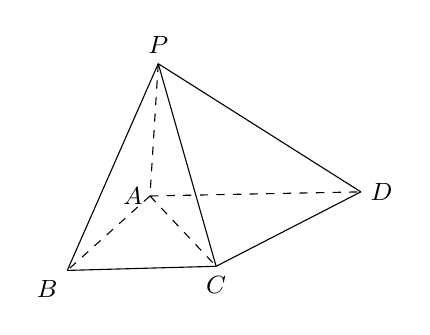
\begin{tikzpicture}[scale=1.05, font=\small]
  \coordinate (P) at (1.45,2.5);
  \coordinate (A) at (1.35,0.9);
  \coordinate (B) at (0.35,0);
  \coordinate (C) at (2.15,0.05);
  \coordinate (D) at (3.9,0.95);
  \draw (P) -- (B)  (P) -- (C)  (P) -- (D);
  \draw (B) -- (C) -- (D);
  \draw[dashed] (P) -- (A);
  \draw[dashed] (A) -- (B)  (A) -- (D)  (A) -- (C);
  \node[above] at (P) {$P$};
  \node[left, inner sep=2.5pt] at (A) {$A$};
  \node[below left] at (B) {$B$};
  \node[below] at (C) {$C$};
  \node[right] at (D) {$D$};
\end{tikzpicture}
\end{center}
\nopagebreak[4]
  (1) 证明：平面 $PAB\perp$ 平面 $PAD$；

  (2) 设 $PA=AB=\sqrt2$，$BC=2$，$AD=1+\sqrt3$，且点 $P$，$B$，$C$，$D$ 均在球 $O$ 的球面上．

  　① 证明：点 $O$ 在平面 $ABCD$ 内；

  　② 求直线 $AC$ 与 $PO$ 所成角的余弦值．

\Needspace{4\baselineskip}
\textbf{解析}

  (1) 证明：平面 $PAB\perp$ 平面 $PAD$；
  (2) 设 $PA=AB=\sqrt2$，$BC=2$，$AD=1+\sqrt3$，且点 $P$，$B$，$C$，$D$ 均在球 $O$ 的球面上。① 证明：点 $O$ 在平面 $ABCD$ 内；② 求直线 $AC$ 与 $PO$ 所成角的余弦值。

\par\medskip

\textbf{(1) 证明}

\Needspace{5\baselineskip}
因为 $PA\perp$ 底面 $ABCD$，而 $AB\subset$ 底面 $ABCD$，所以
\nopagebreak[4]
\[PA\perp AB\]

\Needspace{5\baselineskip}
又已知 $AB\perp AD$，且
\nopagebreak[4]
\[PA\cap AD=A,\qquad PA,\ AD\subset\text{\text{平面} }PAD\]

\Needspace{5\baselineskip}
由\textbf{线面垂直的判定定理}：
\nopagebreak[4]
\[AB\perp\text{\text{平面} }PAD\]

\Needspace{5\baselineskip}
而 $AB\subset$ 平面 $PAB$，由\textbf{面面垂直的判定定理}：
\nopagebreak[4]
\[\text{\text{平面} }PAB\perp\text{\text{平面} }PAD\qquad\blacksquare\]

\par\medskip

\textbf{(2) 解}

\Needspace{5\baselineskip}
\textbf{建系}：由 (1) 的分析，$PA$、$AB$、$AD$ 两两垂直，故以 $A$ 为原点，$AB$、$AD$、$AP$ 分别为 $x$、$y$、$z$ 轴：

\nopagebreak[4]
\[A(0,0,0),\quad B\left(\sqrt2,0,0\right),\quad D\left(0,\ 1+\sqrt3,\ 0\right),\quad P\left(0,0,\sqrt2\right)\]

\Needspace{5\baselineskip}
$C$ 的确定：$BC\parallel AD$ 且 $BC=2$，$AD$ 沿 $y$ 轴正方向，故从 $B$ 出发沿 $y$ 轴正方向走 $2$：
\nopagebreak[4]
\[C\left(\sqrt2,\ 2,\ 0\right)\]

\par\medskip

\textbf{① 证明点 $O$ 在平面 $ABCD$ 内}

设球心 $O(x,y,z)$。由 $O$ 到 $P$、$B$、$C$、$D$ 距离相等，逐一列式。

\Needspace{5\baselineskip}
\textbf{由 $|OB|=|OC|$}（两点横坐标相同，均为 $\sqrt2$；纵坐标分别为 $0$、$2$）：
\nopagebreak[4]
\[(x-\sqrt2)^2+y^2+z^2=(x-\sqrt2)^2+(y-2)^2+z^2\]
\nopagebreak[4]
\[y^2=(y-2)^2\ \Longrightarrow\ 0=-4y+4\ \Longrightarrow\ y=1\]

\Needspace{5\baselineskip}
\textbf{由 $|OB|=|OD|$}（代入 $y=1$）：
\nopagebreak[4]
\[(x-\sqrt2)^2+1^2+z^2=x^2+\left(1-1-\sqrt3\right)^2+z^2\]
\nopagebreak[4]
\[x^2-2\sqrt2x+2+1=x^2+3\]
\nopagebreak[4]
\[-2\sqrt2x=0\ \Longrightarrow\ x=0\]

\Needspace{5\baselineskip}
\textbf{由 $|OP|=|OB|$}（代入 $x=0$，$y=1$）：
\nopagebreak[4]
\[0+1+\left(z-\sqrt2\right)^2=\left(0-\sqrt2\right)^2+1+z^2\]
\nopagebreak[4]
\[1+z^2-2\sqrt2z+2=2+1+z^2\]
\nopagebreak[4]
\[-2\sqrt2z=0\ \Longrightarrow\ z=0\]

\Needspace{5\baselineskip}
故
\nopagebreak[4]
\[O(0,\ 1,\ 0)\]

因为 $O$ 的竖坐标 $z=0$，而平面 $ABCD$ 正是 $z=0$ 平面，所以\textbf{点 $O$ 在平面 $ABCD$ 内}。$\blacksquare$

（可顺带验证半径：$|OB|=\sqrt{2+1}=\sqrt3$，$|OC|=\sqrt{2+1}=\sqrt3$，$|OD|=\sqrt{0+3}=\sqrt3$，$|OP|=\sqrt{0+1+2}=\sqrt3$  四点确实共球面。）

\par\medskip

\Needspace{5\baselineskip}
\textbf{② 求直线 $AC$ 与 $PO$ 所成角的余弦值}

\nopagebreak[4]
\[\overrightarrow{AC}=C-A=\left(\sqrt2,\ 2,\ 0\right),\qquad \overrightarrow{PO}=O-P=\left(0,\ 1,\ -\sqrt2\right)\]

\Needspace{5\baselineskip}
计算：
\nopagebreak[4]
\[\overrightarrow{AC}\cdot\overrightarrow{PO}=\sqrt2\times0+2\times1+0\times\left(-\sqrt2\right)=2\]
\nopagebreak[4]
\[\left|\overrightarrow{AC}\right|=\sqrt{2+4}=\sqrt6,\qquad \left|\overrightarrow{PO}\right|=\sqrt{0+1+2}=\sqrt3\]

\Needspace{5\baselineskip}
设所成角为 $\theta$，\textbf{异面直线所成角必须取绝对值}（角的范围是 $\left(0,\dfrac\pi2\right]$）：
\nopagebreak[4]
\[\cos\theta=\frac{\left|\overrightarrow{AC}\cdot\overrightarrow{PO}\right|}{\left|\overrightarrow{AC}\right|\cdot\left|\overrightarrow{PO}\right|}=\frac{2}{\sqrt6\times\sqrt3}=\frac{2}{\sqrt{18}}=\frac{2}{3\sqrt2}=\frac{\sqrt2}{3}\]

\textbf{所以直线 $AC$ 与 $PO$ 所成角的余弦值为 $\dfrac{\sqrt2}{3}$。}

\begin{gktip}
\textbf{方法总结}：外接球问题的通法就是\textbf{设球心坐标、列等距方程}。本题给出的数据（$AD=1+\sqrt3$ 这种不规则数值）看似奇怪，实则是为了让球心恰好落在底面内——这也正是 ① 要证明的结论。
\end{gktip}

\gkanswer{答案（1）：见解析版}

\gkanswer{答案（2）：② $\dfrac{\sqrt2}{3}$}

\par\medskip

\end{answer}
\begin{answer}
\gksolhead{18}{17 分}

\textbf{题目}（17 分）：

已知椭圆 $C:\dfrac{x^2}{a^2}+\dfrac{y^2}{b^2}=1\ (a>b>0)$ 的离心率为 $\dfrac{2\sqrt2}{3}$，下顶点为 $A$，右顶点为 $B$，$|AB|=\sqrt{10}$．

  (1) 求 $C$ 的方程；

  (2) 已知动点 $P$ 不在 $y$ 轴上，点 $R$ 在射线 $AP$ 上，且满足 $|AP|\cdot|AR|=3$．

  　① 设 $P(m,n)$，求 $R$ 的坐标（用 $m$，$n$ 表示）；

  　② 设 $O$ 为坐标原点，$Q$ 是 $C$ 上的动点，直线 $OR$ 的斜率是直线 $OP$ 的斜率的 $3$ 倍，求 $|PQ|$ 的最大值．

\Needspace{4\baselineskip}
\textbf{解析}

  (1) 求 $C$ 的方程；
  (2) 动点 $P$ 不在 $y$ 轴上，点 $R$ 在射线 $AP$ 上且 $|AP|\cdot|AR|=3$。① 设 $P(m,n)$，求 $R$ 的坐标；② 设 $Q$ 是 $C$ 上的动点，直线 $OR$ 的斜率是直线 $OP$ 的斜率的 $3$ 倍，求 $|PQ|$ 的最大值。

\par\medskip

\textbf{(1) 解}

\Needspace{5\baselineskip}
下顶点 $A(0,-b)$，右顶点 $B(a,0)$，故
\nopagebreak[4]
\[|AB|^2=a^2+b^2=10\qquad\cdots(1)\]

\Needspace{5\baselineskip}
由离心率：
\nopagebreak[4]
\[e^2=\frac{c^2}{a^2}=\frac{a^2-b^2}{a^2}=\left(\frac{2\sqrt2}{3}\right)^2=\frac89\]

\Needspace{5\baselineskip}
即 $9\left(a^2-b^2\right)=8a^2$，化简得
\nopagebreak[4]
\[a^2=9b^2\qquad\cdots(2)\]

\Needspace{5\baselineskip}
把 (2) 代入 (1)：
\nopagebreak[4]
\[9b^2+b^2=10\ \Longrightarrow\ b^2=1,\qquad a^2=9\]

\Needspace{5\baselineskip}
\textbf{所以 $C$ 的方程为}
\nopagebreak[4]
\[\frac{x^2}{9}+y^2=1\]

\par\medskip

\textbf{(2)① 解}

由 (1) 知 $b=1$，故下顶点 $A(0,-1)$。

\Needspace{5\baselineskip}
$R$ 在\textbf{射线} $AP$ 上，故存在 $\lambda>0$ 使
\nopagebreak[4]
\[\overrightarrow{AR}=\lambda\,\overrightarrow{AP}\]

\Needspace{5\baselineskip}
于是 $|AR|=\lambda|AP|$，代入条件 $|AP|\cdot|AR|=3$：
\nopagebreak[4]
\[\lambda\left|AP\right|^2=3\ \Longrightarrow\ \lambda=\frac{3}{\left|AP\right|^2}\]

\Needspace{5\baselineskip}
而 $\overrightarrow{AP}=(m,\ n+1)$，$\left|AP\right|^2=m^2+(n+1)^2$，故
\nopagebreak[4]
\[\lambda=\frac{3}{m^2+(n+1)^2}\]

\Needspace{5\baselineskip}
因此
\nopagebreak[4]
\[R=A+\lambda\overrightarrow{AP}=\left(0,-1\right)+\frac{3}{m^2+(n+1)^2}\left(m,\ n+1\right)\]

\nopagebreak[4]
\[\boxed{R\left(\ \frac{3m}{m^2+(n+1)^2},\ \ -1+\frac{3(n+1)}{m^2+(n+1)^2}\ \right)}\]

\begin{gktip}
这个变换在几何上叫\textbf{以 $A$ 为中心、幂为 $3$ 的反演}。
\end{gktip}

\par\medskip

\textbf{(2)② 解}

\textbf{第一步，把斜率条件化为 $P$ 的轨迹方程（本问的关键）。}

\Needspace{5\baselineskip}
记 $D=m^2+(n+1)^2>0$（$P$ 不在 $y$ 轴上保证 $m\ne0$，故 $D>0$）。由 ①：
\nopagebreak[4]
\[x_R=\frac{3m}{D},\qquad y_R=-1+\frac{3(n+1)}{D}=\frac{-D+3(n+1)}{D}\]

\Needspace{5\baselineskip}
于是
\nopagebreak[4]
\[k_{OR}=\frac{y_R}{x_R}=\frac{-D+3(n+1)}{3m},\qquad k_{OP}=\frac nm\]

\Needspace{5\baselineskip}
由 $k_{OR}=3k_{OP}$：
\nopagebreak[4]
\[\frac{-D+3(n+1)}{3m}=\frac{3n}{m}\]

\Needspace{5\baselineskip}
两边乘 $3m$（$m\ne0$）：
\nopagebreak[4]
\[-D+3n+3=9n\ \Longrightarrow\ D=3-6n\]

\Needspace{5\baselineskip}
代回 $D$ 的定义：
\nopagebreak[4]
\[m^2+(n+1)^2=3-6n\]
\nopagebreak[4]
\[m^2+n^2+2n+1=3-6n\]
\nopagebreak[4]
\[m^2+n^2+8n-2=0\]

\Needspace{5\baselineskip}
配方：
\nopagebreak[4]
\[m^2+(n+4)^2=18\]

\textbf{结论}：动点 $P$ 的轨迹是以 $O'(0,-4)$ 为圆心、$r=3\sqrt2$ 为半径的\textbf{圆}（去掉与 $y$ 轴的交点）。

\textbf{第二步，求 $|PQ|$ 的最大值。}

\Needspace{5\baselineskip}
$Q$ 在椭圆 $\dfrac{x^2}{9}+y^2=1$ 上，$P$ 在上述圆上。由三角形不等式：
\nopagebreak[4]
\[|PQ|\le|QO'|+|O'P|=|QO'|+3\sqrt2\]

等号当 $P$ 位于射线 $QO'$ 的延长线与圆的交点时取到。

因此只需\textbf{最大化 $|QO'|$}（$Q$ 在椭圆上，$O'(0,-4)$ 固定）。

\Needspace{5\baselineskip}
设 $Q\left(3\cos\theta,\ \sin\theta\right)$：
\nopagebreak[4]
\[|QO'|^2=9\cos^2\theta+(\sin\theta+4)^2\]

\Needspace{5\baselineskip}
用 $\cos^2\theta=1-\sin^2\theta$ 统一为 $\sin\theta$ 的二次式：
\nopagebreak[4]
\[=9-9\sin^2\theta+\sin^2\theta+8\sin\theta+16=-8\sin^2\theta+8\sin\theta+25\]

\Needspace{5\baselineskip}
令 $s=\sin\theta\in[-1,1]$，$g(s)=-8s^2+8s+25$，对称轴
\nopagebreak[4]
\[s=\frac{-8}{2\times(-8)}=\frac12\in[-1,1]\]

\nopagebreak[4]
\[g\left(\frac12\right)=-8\times\frac14+8\times\frac12+25=-2+4+25=27\]

故 $|QO'|_{\max}=\sqrt{27}=3\sqrt3$。

\Needspace{5\baselineskip}
\textbf{第三步，作答并验证等号可取。}

\nopagebreak[4]
\[|PQ|_{\max}=3\sqrt3+3\sqrt2\]

\textbf{验证}：$s=\sin\theta=\dfrac12$ 时 $\cos\theta=\pm\dfrac{\sqrt3}{2}$，取 $Q\left(\dfrac{3\sqrt3}{2},\ \dfrac12\right)$。直线 $QO'$ 不竖直，故它与圆的两个交点横坐标均不为 $0$，即所需的 $P$ 满足「不在 $y$ 轴上」的限制  等号可以取到。

\textbf{所以 $|PQ|$ 的最大值为 $3\sqrt3+3\sqrt2$。}

\begin{gktip}
\textbf{方法总结}：本题层层递进——① 把几何条件（反演）写成坐标；② 把斜率条件\textbf{化简为轨迹方程}（发现 $P$ 在一个圆上，这是转折点）；③ 「圆上点到椭圆上点的最大距离」用三角形不等式拆成「圆心到椭圆的最大距离 $+$ 半径」；④ 椭圆上点到定点的距离用\textbf{参数方程}化为二次函数求最值。每一步都是常见套路，难在组合。
\end{gktip}

\gkanswer{答案（1）：$\dfrac{x^2}{9}+y^2=1$}

\gkanswer{答案（2）：① $R\left(\frac{3m}{m^2+(n+1)^2},\ \ -1+\frac{3(n+1)}{m^2+(n+1)^2}\right)$；② $|PQ|_{\max}=3\sqrt3+3\sqrt2$}

\par\medskip

\end{answer}
\begin{answer}
\gksolhead{19}{17 分}

\textbf{题目}（17 分）：

(1) 求函数 $f(x)=5\cos x-\cos 5x$ 在区间 $\left[0,\dfrac{\pi}{4}\right]$ 的最大值；

  (2) 给定 $\theta\in(0,\pi)$ 和 $a\in\mathbf{R}$，证明：存在 $y\in[a-\theta,\ a+\theta]$ 使得 $\cos y\le\cos\theta$；

  (3) 设 $b\in\mathbf{R}$，若存在 $\varphi\in\mathbf{R}$ 使得 $5\cos x-\cos(5x+\varphi)\le b$ 对 $x\in\mathbf{R}$ 恒成立，求 $b$ 的最小值．

\par\medskip

\Needspace{4\baselineskip}
\textbf{解析}

  (1) 求函数 $f(x)=5\cos x-\cos5x$ 在区间 $\left[0,\dfrac\pi4\right]$ 的最大值；
  (2) 给定 $\theta\in(0,\pi)$ 和 $a\in\mathbf R$，证明：存在 $y\in[a-\theta,\ a+\theta]$ 使得 $\cos y\le\cos\theta$；
  (3) 设 $b\in\mathbf R$，若存在 $\varphi\in\mathbf R$ 使得 $5\cos x-\cos(5x+\varphi)\le b$ 对 $x\in\mathbf R$ 恒成立，求 $b$ 的最小值。

\par\medskip

\Needspace{5\baselineskip}
\textbf{(1) 解}

\nopagebreak[4]
\[f'(x)=-5\sin x+5\sin5x=5\left(\sin5x-\sin x\right)\]

\Needspace{5\baselineskip}
令 $f'(x)=0$，即 $\sin5x=\sin x$，解为
\nopagebreak[4]
\[5x=x+2k\pi\ \ \text{\text{或}}\ \ 5x=\pi-x+2k\pi\]

\Needspace{5\baselineskip}
即
\nopagebreak[4]
\[x=\frac{k\pi}{2}\qquad\text{\text{或}}\qquad x=\frac{(2k+1)\pi}{6}\]

\Needspace{5\baselineskip}
在区间 $\left[0,\dfrac\pi4\right]$（约 $[0,\ 0.785]$）内的临界点与端点为
\nopagebreak[4]
\[x=0,\qquad x=\frac\pi6\approx0.524,\qquad x=\frac\pi4\]

\Needspace{5\baselineskip}
逐一计算：

\nopagebreak[4]
\[f(0)=5\times1-\cos0=5-1=4\]

\nopagebreak[4]
\[f\left(\frac\pi6\right)=5\cos\frac\pi6-\cos\frac{5\pi}6=5\times\frac{\sqrt3}{2}-\left(-\frac{\sqrt3}{2}\right)=\frac{5\sqrt3}{2}+\frac{\sqrt3}{2}=3\sqrt3\]

\nopagebreak[4]
\[f\left(\frac\pi4\right)=5\cos\frac\pi4-\cos\frac{5\pi}4=5\times\frac{\sqrt2}{2}-\left(-\frac{\sqrt2}{2}\right)=\frac{5\sqrt2}{2}+\frac{\sqrt2}{2}=3\sqrt2\]

比较：$3\sqrt3\approx5.196>4>3\sqrt2\approx4.243$。

\textbf{所以最大值为 $3\sqrt3$。}

\par\medskip

\textbf{(2) 证明}

\textbf{思路：比较区间长度。}

\Needspace{5\baselineskip}
先刻画使 $\cos y>\cos\theta$ 的 $y$ 的集合。由于 $\theta\in(0,\pi)$，在一个周期 $[-\pi,\pi]$ 内 $\cos y>\cos\theta\iff|y|<\theta$。推广到全体实数：
\nopagebreak[4]
\[\left\{y\mid\cos y>\cos\theta\right\}=\bigcup_{k\in\mathbb Z}\left(2k\pi-\theta,\ 2k\pi+\theta\right)\]

这是一族\textbf{开区间}，每个长度恰为 $2\theta$。

\textbf{反证法。} 假设结论不成立，即对一切 $y\in[a-\theta,a+\theta]$ 都有 $\cos y>\cos\theta$，那么整个闭区间被包含在上述并集里。

\Needspace{5\baselineskip}
由于闭区间 $[a-\theta,a+\theta]$ 是\textbf{连通}的，而各开区间互不相交（相邻两个的间隔为 $2\pi-2\theta>0$），故它必须整个落入\textbf{某一个}开区间：
\nopagebreak[4]
\[[a-\theta,\ a+\theta]\subseteq\left(2k\pi-\theta,\ 2k\pi+\theta\right)\]

\Needspace{5\baselineskip}
比较端点：
\nopagebreak[4]
\[a-\theta>2k\pi-\theta\ \Longrightarrow\ a>2k\pi\]
\nopagebreak[4]
\[a+\theta<2k\pi+\theta\ \Longrightarrow\ a<2k\pi\]

两式\textbf{矛盾}（$a$ 不能既大于又小于 $2k\pi$）。

\textbf{根本原因}：闭区间与开区间\textbf{长度相同}（都是 $2\theta$），长度相同的闭区间不可能真包含于开区间。

故假设不成立，即存在 $y\in[a-\theta,\ a+\theta]$ 使得 $\cos y\le\cos\theta$。$\blacksquare$

\par\medskip

\textbf{(3) 解}

\Needspace{5\baselineskip}
记 $g(x)=5\cos x-\cos(5x+\varphi)$。题目要求找出最小的 $b$，使得\textbf{存在}某个 $\varphi$ 让 $g(x)\le b$ 恒成立，即
\nopagebreak[4]
\[b_{\min}=\min_{\varphi\in\mathbf R}\ \max_{x\in\mathbf R}\ g(x)\]

\textbf{第一步：证明下界 $\max_x g(x)\ge3\sqrt3$ 对一切 $\varphi$ 成立。}

这一步正是 (2) 的用武之地。

\Needspace{5\baselineskip}
任取 $\theta\in(0,\pi)$。当 $x$ 在区间 $\left[-\dfrac\theta5,\ \dfrac\theta5\right]$ 上变化时，$5x+\varphi$ 恰好\textbf{跑遍}区间
\nopagebreak[4]
\[\left[\varphi-\theta,\ \varphi+\theta\right]\]

\Needspace{5\baselineskip}
由 (2)（取 $a=\varphi$），存在 $y_0\in[\varphi-\theta,\varphi+\theta]$ 使 $\cos y_0\le\cos\theta$。设其对应的
\nopagebreak[4]
\[x_0=\frac{y_0-\varphi}{5}\in\left[-\frac\theta5,\ \frac\theta5\right]\]

\Needspace{5\baselineskip}
于是
\nopagebreak[4]
\[g(x_0)=5\cos x_0-\cos y_0\ \ge\ 5\cos x_0-\cos\theta\]

\Needspace{5\baselineskip}
又 $|x_0|\le\dfrac\theta5<\dfrac\pi5<\dfrac\pi2$，余弦在 $\left[0,\dfrac\pi2\right]$ 递减且为偶函数，故 $\cos x_0\ge\cos\dfrac\theta5$：
\nopagebreak[4]
\[\max_{x}g(x)\ \ge\ g(x_0)\ \ge\ 5\cos\frac\theta5-\cos\theta\]

\Needspace{5\baselineskip}
\textbf{这个下界对一切 $\theta\in(0,\pi)$ 都成立}，因此可以取右端的最大值。令
\nopagebreak[4]
\[h(\theta)=5\cos\frac\theta5-\cos\theta\]
\nopagebreak[4]
\[h'(\theta)=-\sin\frac\theta5+\sin\theta=0\ \Longrightarrow\ \sin\theta=\sin\frac\theta5\]

\Needspace{5\baselineskip}
在 $(0,\pi)$ 内解 $\theta=\pi-\dfrac\theta5$，得 $\dfrac{6\theta}{5}=\pi$，即
\nopagebreak[4]
\[\theta=\frac{5\pi}{6}\]

\nopagebreak[4]
\[h\left(\frac{5\pi}{6}\right)=5\cos\frac\pi6-\cos\frac{5\pi}6=\frac{5\sqrt3}{2}+\frac{\sqrt3}{2}=3\sqrt3\]

\Needspace{5\baselineskip}
故对任意 $\varphi$：
\nopagebreak[4]
\[\max_x g(x)\ \ge\ 3\sqrt3\qquad\Longrightarrow\qquad b\ge3\sqrt3\]

\textbf{第二步：证明 $b=3\sqrt3$ 可以取到（取 $\varphi=0$）。}

此时 $g(x)=5\cos x-\cos5x$，即 (1) 中的 $f(x)$。它以 $2\pi$ 为周期且为偶函数，故只需考察 $[0,\pi]$。

临界点为 $x=0,\ \dfrac\pi6,\ \dfrac\pi2,\ \dfrac{5\pi}6,\ \pi$：

\begin{center}
\begin{tabular}{cccccc}
\toprule
$x$ & $0$ & $\dfrac\pi6$ & $\dfrac\pi2$ & $\dfrac{5\pi}6$ & $\pi$ \\
\midrule
$f(x)$ & $4$ & $3\sqrt3$ & $0$ & $-3\sqrt3$ & $-4$ \\
\bottomrule
\end{tabular}
\end{center}

\Needspace{5\baselineskip}
最大值为 $3\sqrt3$，即
\nopagebreak[4]
\[5\cos x-\cos5x\le3\sqrt3\quad\text{\text{对一切} }x\in\mathbf R\text{ \text{成立}}\]

\Needspace{5\baselineskip}
\textbf{结论}：$b$ 的最小值为
\nopagebreak[4]
\[\boxed{3\sqrt3}\]

\Needspace{24\baselineskip}

\begin{gktip}
\textbf{方法总结}：这是一道结构精巧的三小问递进题——(1) 算出一个具体最大值 $3\sqrt3$（提供\textbf{上界}的候选），(2) 提供一个看似无关的存在性引理，(3) 用该引理证明\textbf{下界}也是 $3\sqrt3$，上下夹逼得到答案。

(2) 的作用值得细品：它保证「无论把 $\cos(5x+\varphi)$ 的相位 $\varphi$ 怎么调，都躲不开一个使 $\cos$ 值足够小的点」，从而 $\varphi$ 的自由度\textbf{帮不上忙}。这类「$\min_\varphi\max_x$」问题的标准思路正是：先证下界对一切参数成立，再举出达到下界的具体参数。
\end{gktip}

\gkanswer{答案（1）：$3\sqrt3$}

\gkanswer{答案（2）：见解析版}

\gkanswer{答案（3）：$b_{\min}=3\sqrt3$}

\end{answer}